% 2008 年北京卷理科第 8 题的四个候选图象：(A) 梯形、(B) 三角形、(C) 不对称梯形、(D) 钟形曲线。
% 来源 PDF、SHA-256 同 q8_cube。
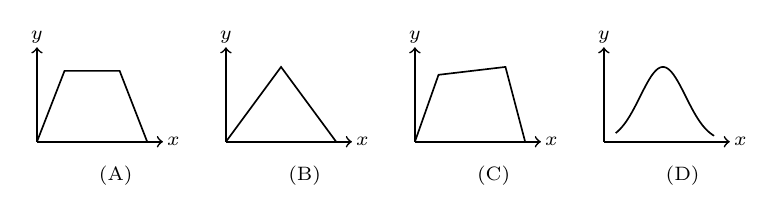
\begin{tikzpicture}[semithick, every node/.style={inner sep=1.2pt}]
  % (A)
  \begin{scope}[shift={(0,0)}]
    \draw[->] (0,0) -- (1.6,0) node[right,font=\scriptsize] {$x$};
    \draw[->] (0,0) -- (0,1.2) node[above,font=\scriptsize] {$y$};
    \draw (0,0) -- (0.35,0.9) -- (1.05,0.9) -- (1.4,0);
    \node[below,font=\scriptsize] at (1.0,-0.25) {(A)};
  \end{scope}
  % (B)
  \begin{scope}[shift={(2.4,0)}]
    \draw[->] (0,0) -- (1.6,0) node[right,font=\scriptsize] {$x$};
    \draw[->] (0,0) -- (0,1.2) node[above,font=\scriptsize] {$y$};
    \draw (0,0) -- (0.7,0.95) -- (1.4,0);
    \node[below,font=\scriptsize] at (1.0,-0.25) {(B)};
  \end{scope}
  % (C)
  \begin{scope}[shift={(4.8,0)}]
    \draw[->] (0,0) -- (1.6,0) node[right,font=\scriptsize] {$x$};
    \draw[->] (0,0) -- (0,1.2) node[above,font=\scriptsize] {$y$};
    \draw (0,0) -- (0.3,0.85) -- (1.15,0.95) -- (1.4,0);
    \node[below,font=\scriptsize] at (1.0,-0.25) {(C)};
  \end{scope}
  % (D)
  \begin{scope}[shift={(7.2,0)}]
    \draw[->] (0,0) -- (1.6,0) node[right,font=\scriptsize] {$x$};
    \draw[->] (0,0) -- (0,1.2) node[above,font=\scriptsize] {$y$};
    \draw[domain=0.15:1.4, samples=50] plot (\x,{0.95*exp(-6*(\x-0.75)*(\x-0.75))});
    \node[below,font=\scriptsize] at (1.0,-0.25) {(D)};
  \end{scope}
\end{tikzpicture}
